\documentclass[11pt]{article}
\usepackage[latin1]{inputenc}
\usepackage{a4wide}
\usepackage{amsmath}
\usepackage{amsfonts}
\usepackage{amssymb}
\usepackage{graphicx}
\usepackage{enumerate}
\usepackage{epstopdf}
\usepackage{float}
\usepackage{multicol}
\usepackage{hyperref}
\epstopdfsetup{outdir=./images/}
\usepackage{subcaption}

\title{Natural Computing, Assignment 2}
\author{Dennis Verheijden - s4455770 \and Pauline Lauron - s1016609 \and Joost Besseling - s4796799}
\begin{document}
\maketitle

\section{Using the Negative Selection Algorithm}
\begin{enumerate}[1.]
\item The ROC curve for the parameters $n=10, r=4$ may be observed in figure \ref{fig:ROC_ex1} as the orange line. The corresponding AUC is 0.7835, which is actually pretty good. The algorithm definitely learned whether the language is English or not.

\item The ROC curves for the parameters $r=1$ and $r=9$ are shown in figure \ref{fig:ROC_ex1} as respectively the green and blue line. Changing the length of the substrings ($r$), we can see some interesting results. If the length is 9, the anomaly scores were constant, so the accuracy, as may be seen the figure, are bad. If the length is 1, it cannot distinguish anything because it has to judge the language given 1 character. This is reflected in the figure, as the ROC curve reflects the baseline, which just guesses.

\begin{figure}[H]
\centering
\includegraphics[width=0.7\textwidth]{images/roc_ex1.eps}
\caption{ROC curve for different values of $r$ in the negative selection algorithm}
\label{fig:ROC_ex1}
\end{figure}

\newpage

\item The ROC curve for differentiation of English and four other languages using the negative selection algorithm may be found in figure \ref{fig:ROC_ex1_3}. What we can see from this figure is that there is a clear ordering which language is discriminated best, since the ROC curves never cross paths, i.e. for every threshold it holds that languages have a constant ordering which is language is discriminated best. Judging from this figure \textit{Xhosa} is discriminated best, followed by respectively \textit{Hiligaynon}, \textit{Plautdietsch} and lastly \textit{Middle-English}.

I was actually suprised that all of the languages, exception being Middle-English, exist. However, upon closer inspection, this ordering makes sense. Middle-English is a precursor of English, so it shares similarities. \textit{Xhosa} is a Nguni Bantu language with `click consonants', so it makes sense that these languages are the most different and thus easiest to distinguish.

\begin{figure}[H]
\centering
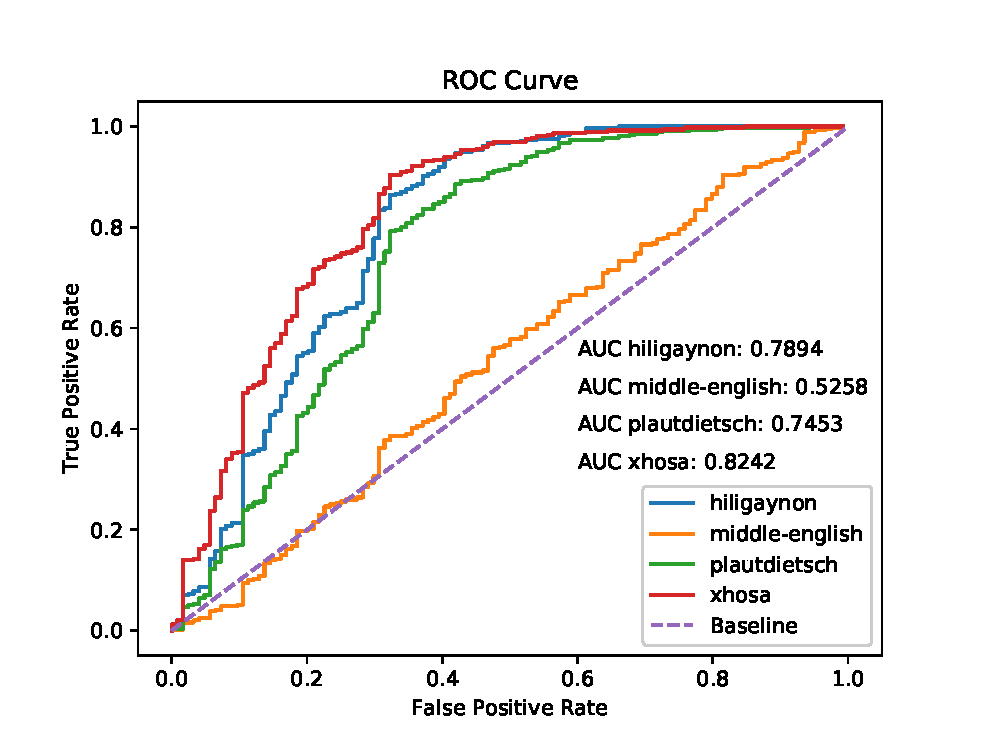
\includegraphics[width=0.7\textwidth]{images/roc_ex1_3.eps}
\caption{ROC curve for differentiation of English and four other languages using the negative selection algorithm.}
\label{fig:ROC_ex1_3}
\end{figure}

\end{enumerate}

\newpage

\section{Intrusion Detection for Unix Processes}
In this exercise we used the negative-selection algorithm to detect anomalous system call sequences. For this we had to change the command with which we call the function to include the new alphabet and point it to the correct files.

When inspecting our training- and test-files, we noticed that there were some sequences that have less than 10 characters. To accommodate for this (such that the algorithm does not produce \textit{NaN} values, we changed the $n$ to the minimal length, which was 7.

After processing the dataset, such that we got the same format as in exercise 1, we ran the algorithm. The resulting anomaly scores were averaged over one instance. We ran the algorithm for two different \textit{syscalls}: \textit{snd-cert} (figure \ref{fig:ROC_ex2_1}) and \textit{snd-unm} (figure \ref{fig:ROC_ex2_2}).

After doing some AUC analysis on these results and tweaking with parameters, we found that the parameter setup $n=7, r=4$ worked best. For both syscalls, the algorithm have a fairly high TPR right off the bat. For \textit{snd-cert} we do not see any significant differences, their AUCs are also the same. Where in \textit{snd-unm} we see some differences: \textit{snd-unm.1} is classified worse than \textit{snd-unm.2} or \textit{snd-unm.3}. This may be due to that the test file being so small.

Overall we can say that the algorithm performs pretty well for this dataset, as it has a high TPR while maintaining a low FPR.


\begin{figure}[H]
\centering
    \begin{subfigure}[b]{0.49\textwidth}
        \includegraphics[width=\textwidth]{images/roc_ex2_1.eps}
        \caption{\textit{snd-cert}}
        \label{fig:ROC_ex2_1}
    \end{subfigure}
    \begin{subfigure}[b]{0.49\textwidth}
        \includegraphics[width=\textwidth]{images/roc_ex2_2.eps}
        \caption{\textit{snd-unm}}
        \label{fig:ROC_ex2_2}
    \end{subfigure}
    \caption{ROC curves for discriminating between genuine and anomalous system calls.}
\end{figure}
\end{document}